\documentclass[11pt]{article}

\usepackage[margin=1in]{geometry}
\usepackage{graphicx}
\usepackage{float}
\usepackage{hyperref}
\usepackage{booktabs}
\usepackage{amsmath}
\usepackage{xcolor}

\title{CS285 HW3 Report\\Q-Learning and Actor-Critic Algorithms}
\author{Qipeng Kong}
\date{\today}

\begin{document}
\maketitle

\section{Deep Q-Learning}

\subsection{Basic DQN on CartPole-v1}
I implemented the standard DQN update with a target network and epsilon-greedy exploration. On CartPole-v1, the agent reached a return of 500 in at least one evaluation rollout, satisfying the assignment sanity check, although the average evaluation return remained below 500.

\begin{figure}[H]
    \centering
    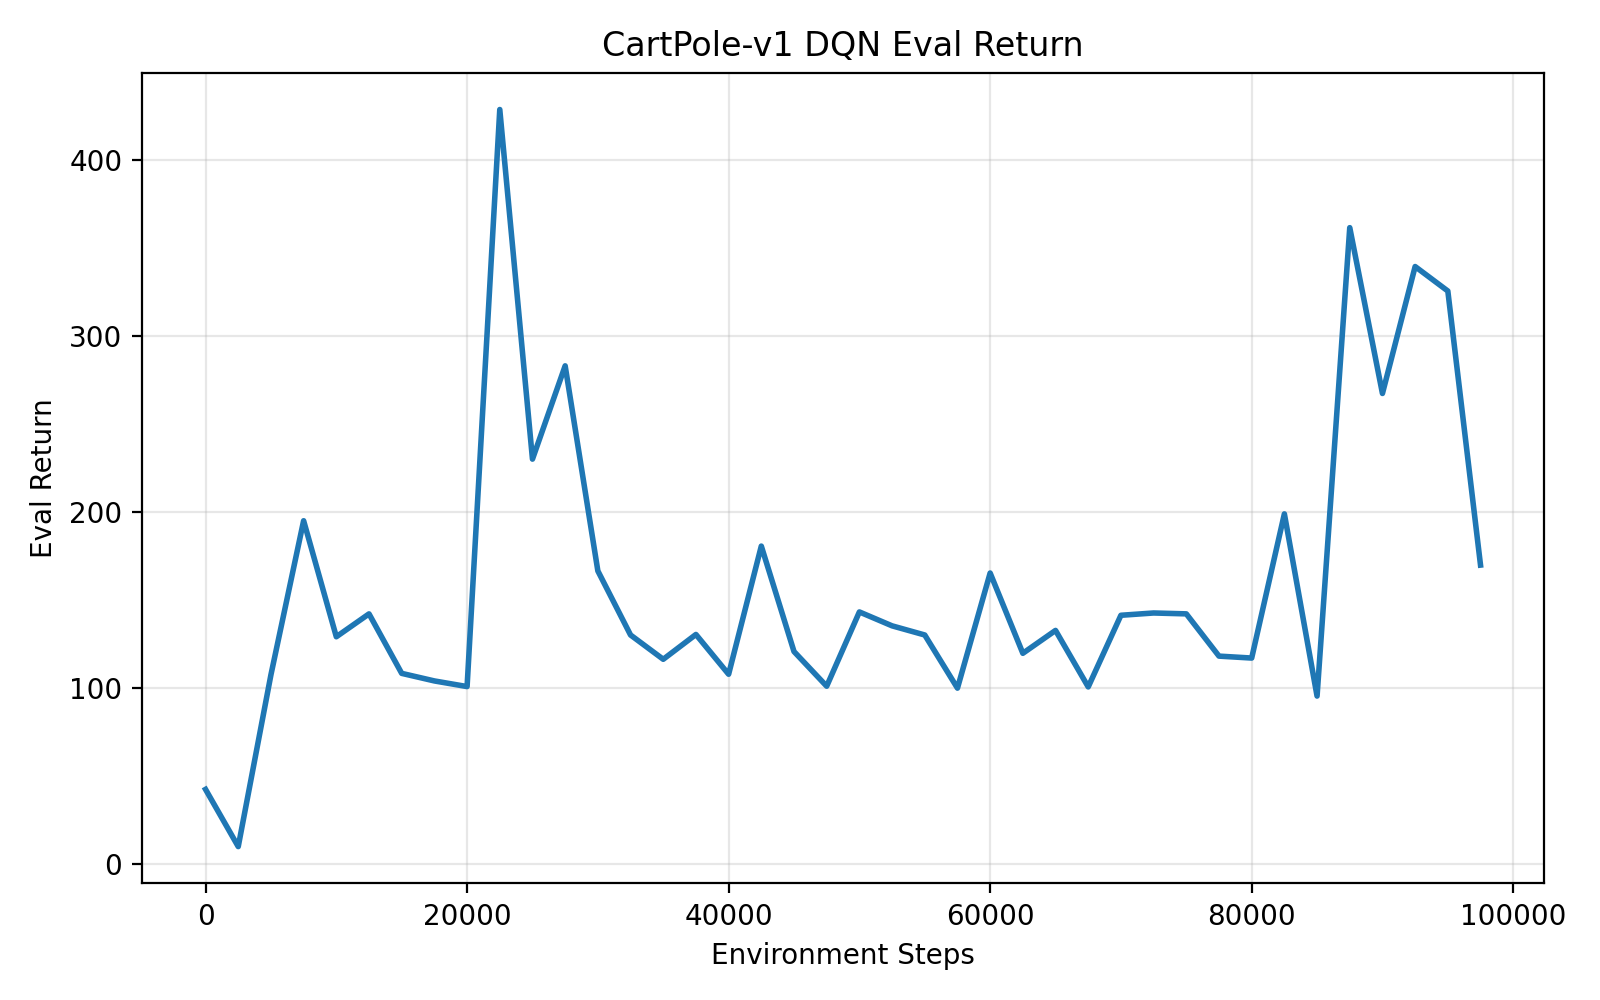
\includegraphics[width=0.8\linewidth]{CartPole-v1_dqn_sd1_20260310_000416_eval_return.png}
    \caption{CartPole-v1 DQN evaluation return versus environment steps.}
\end{figure}

\subsection{Double DQN on LunarLander-v2}
I enabled the double-Q target by selecting the bootstrap action with the online network and evaluating it with the target network. On LunarLander-v2, the resulting agent exceeded the target return of 200 and achieved a best evaluation return of approximately 248.5.

\begin{figure}[H]
    \centering
    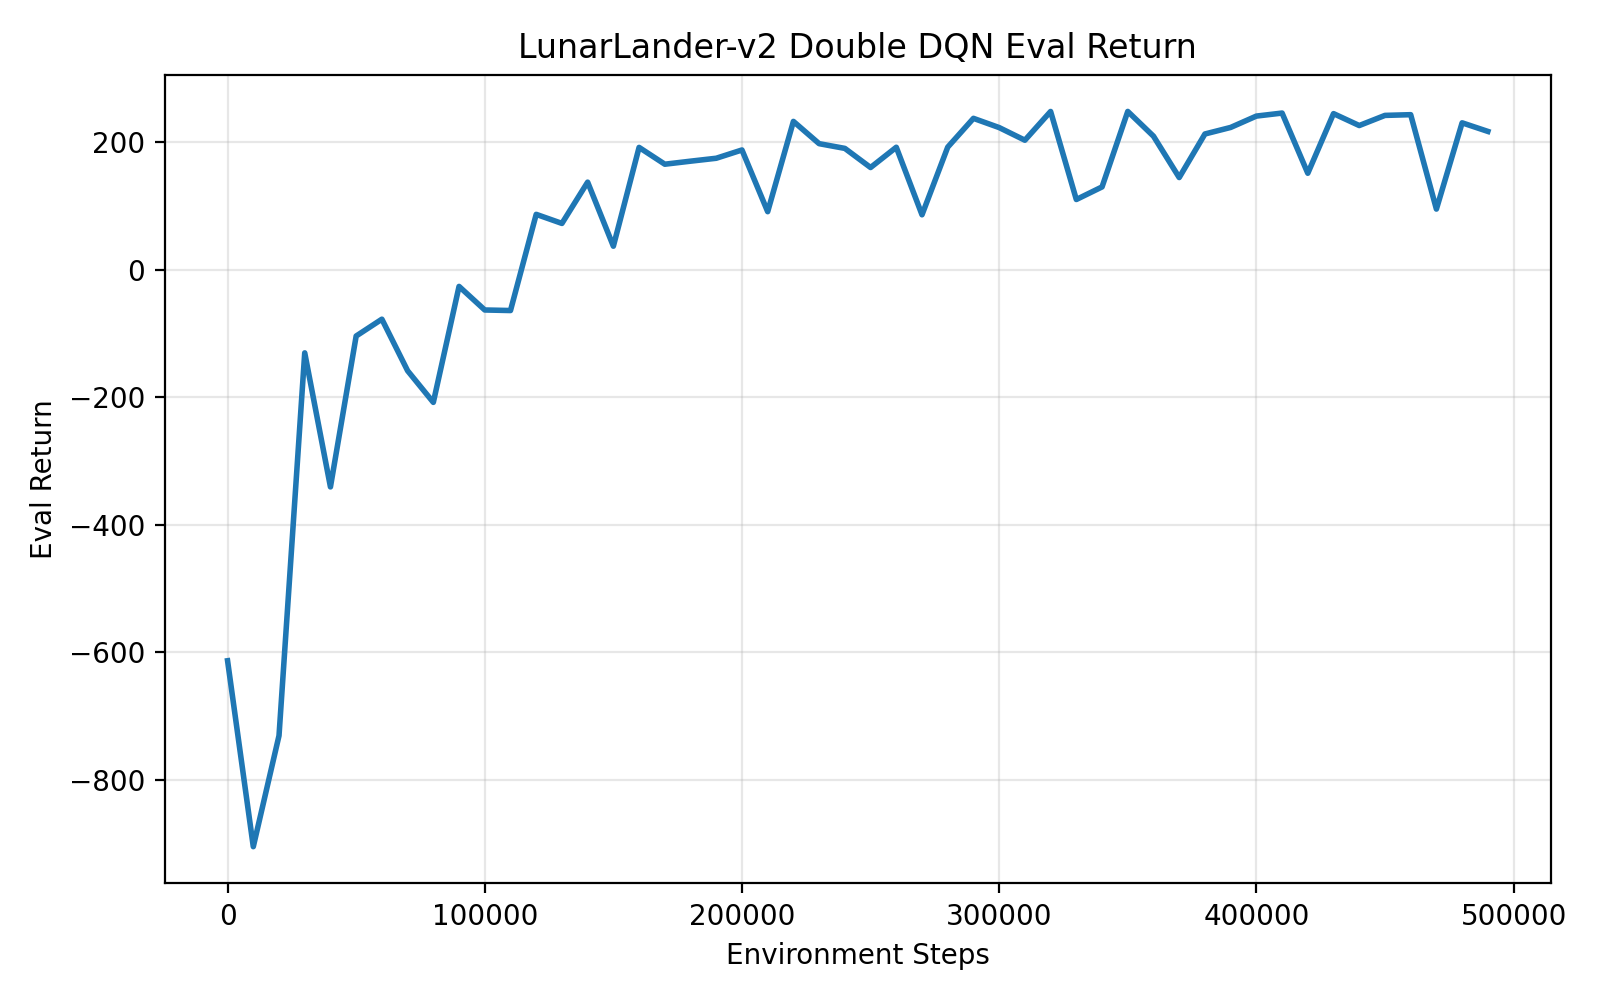
\includegraphics[width=0.8\linewidth]{report_lunarlander_eval_return.png}
    \caption{LunarLander-v2 Double DQN evaluation return versus environment steps.}
\end{figure}

\subsection{MsPacman-v0}
I trained DQN with the provided Atari configuration, which includes double Q-learning, frame stacking, gradient clipping, and the provided exploration and learning-rate schedules. The final run achieved a best evaluation return of 4222, which is well above the assignment target of around 1500.

\begin{figure}[H]
    \centering
    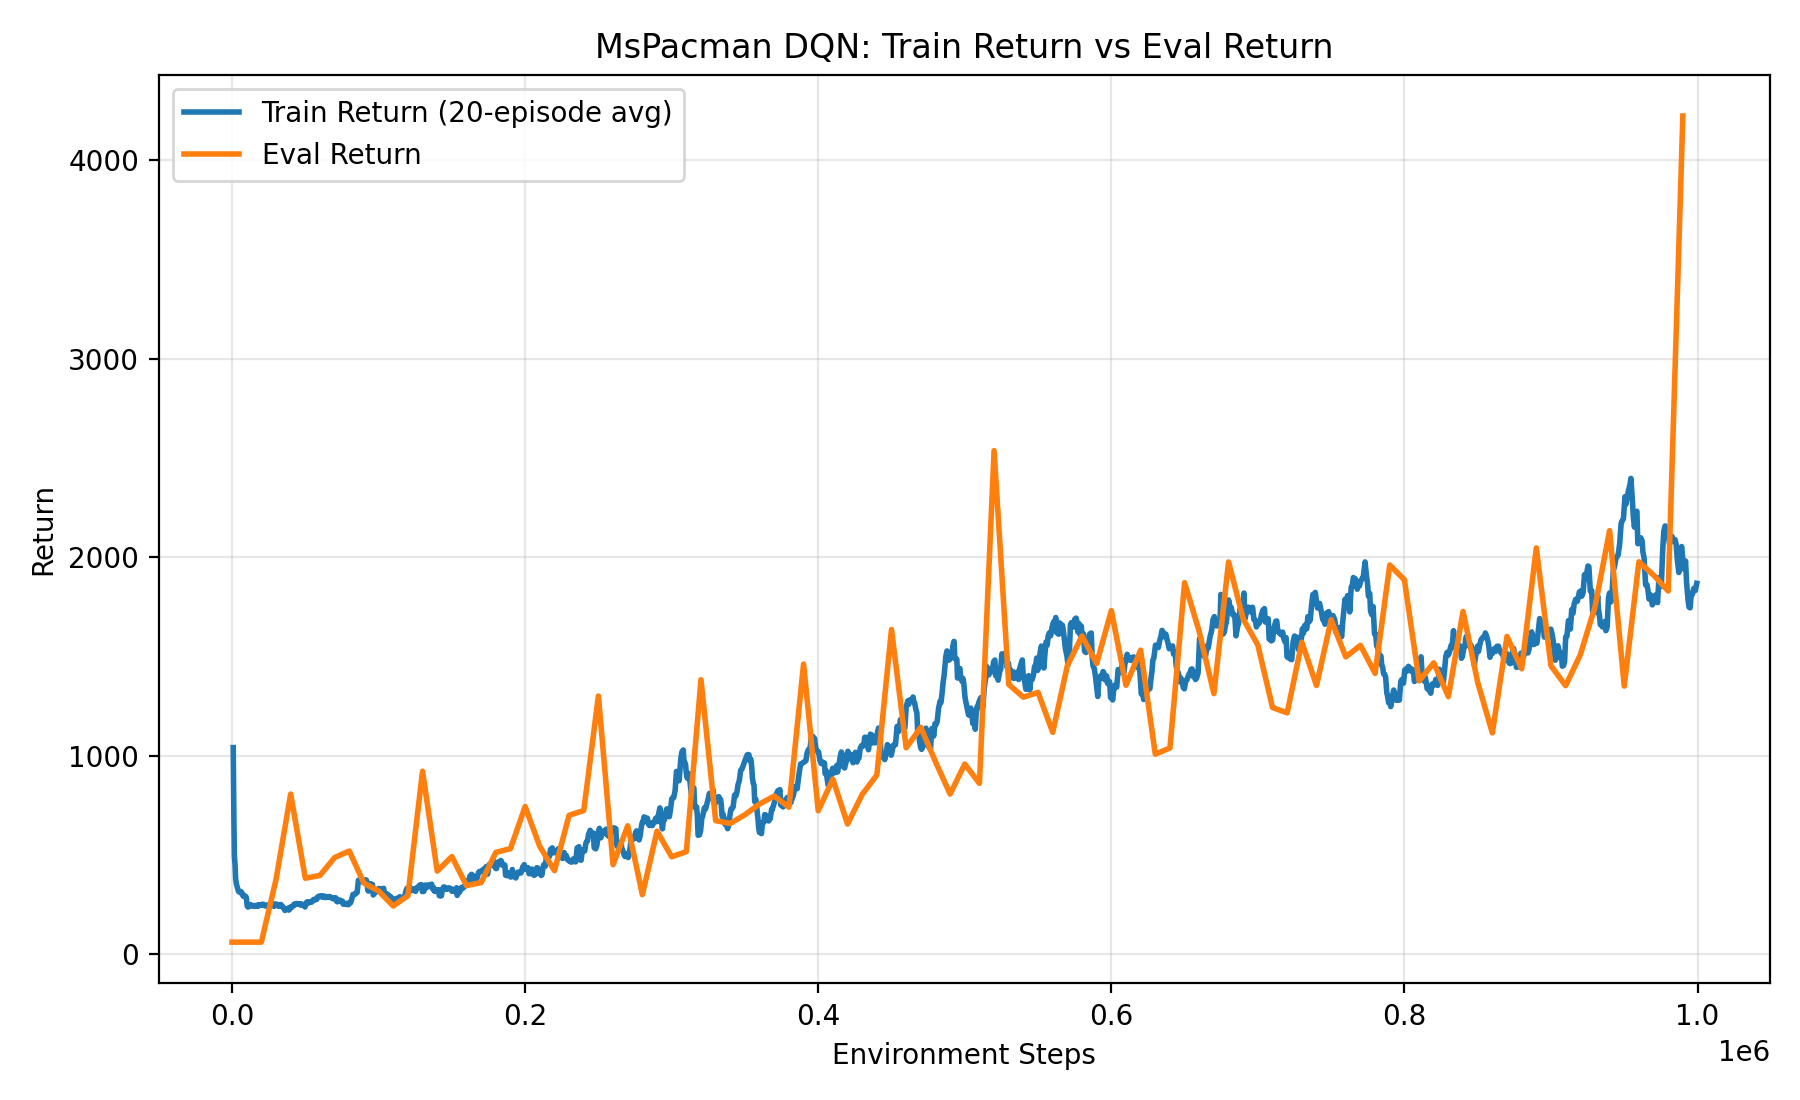
\includegraphics[width=0.9\linewidth]{report_mspacman_train_vs_eval.png}
    \caption{MsPacman-v0 training return and evaluation return on the same axes.}
\end{figure}

Early in training, the training and evaluation curves differ because they are collected under different policies. Training return comes from the epsilon-greedy behavior policy, so it includes random exploratory actions and is therefore noisier. Evaluation return is measured using the greedy policy without exploration, so it reflects the quality of the learned Q-network more directly. As epsilon decays and the agent improves, the two curves become more aligned, although evaluation remains spikier because Atari returns have high variance and are measured less frequently.

\subsection{Hyperparameter Sensitivity on LunarLander-v2}
For the hyperparameter sweep, I varied the learning rate and kept the rest of the configuration fixed. I chose learning rate because it directly affects both optimization stability and sample efficiency in DQN, making it a natural single-parameter probe of training sensitivity.

\begin{figure}[H]
    \centering
    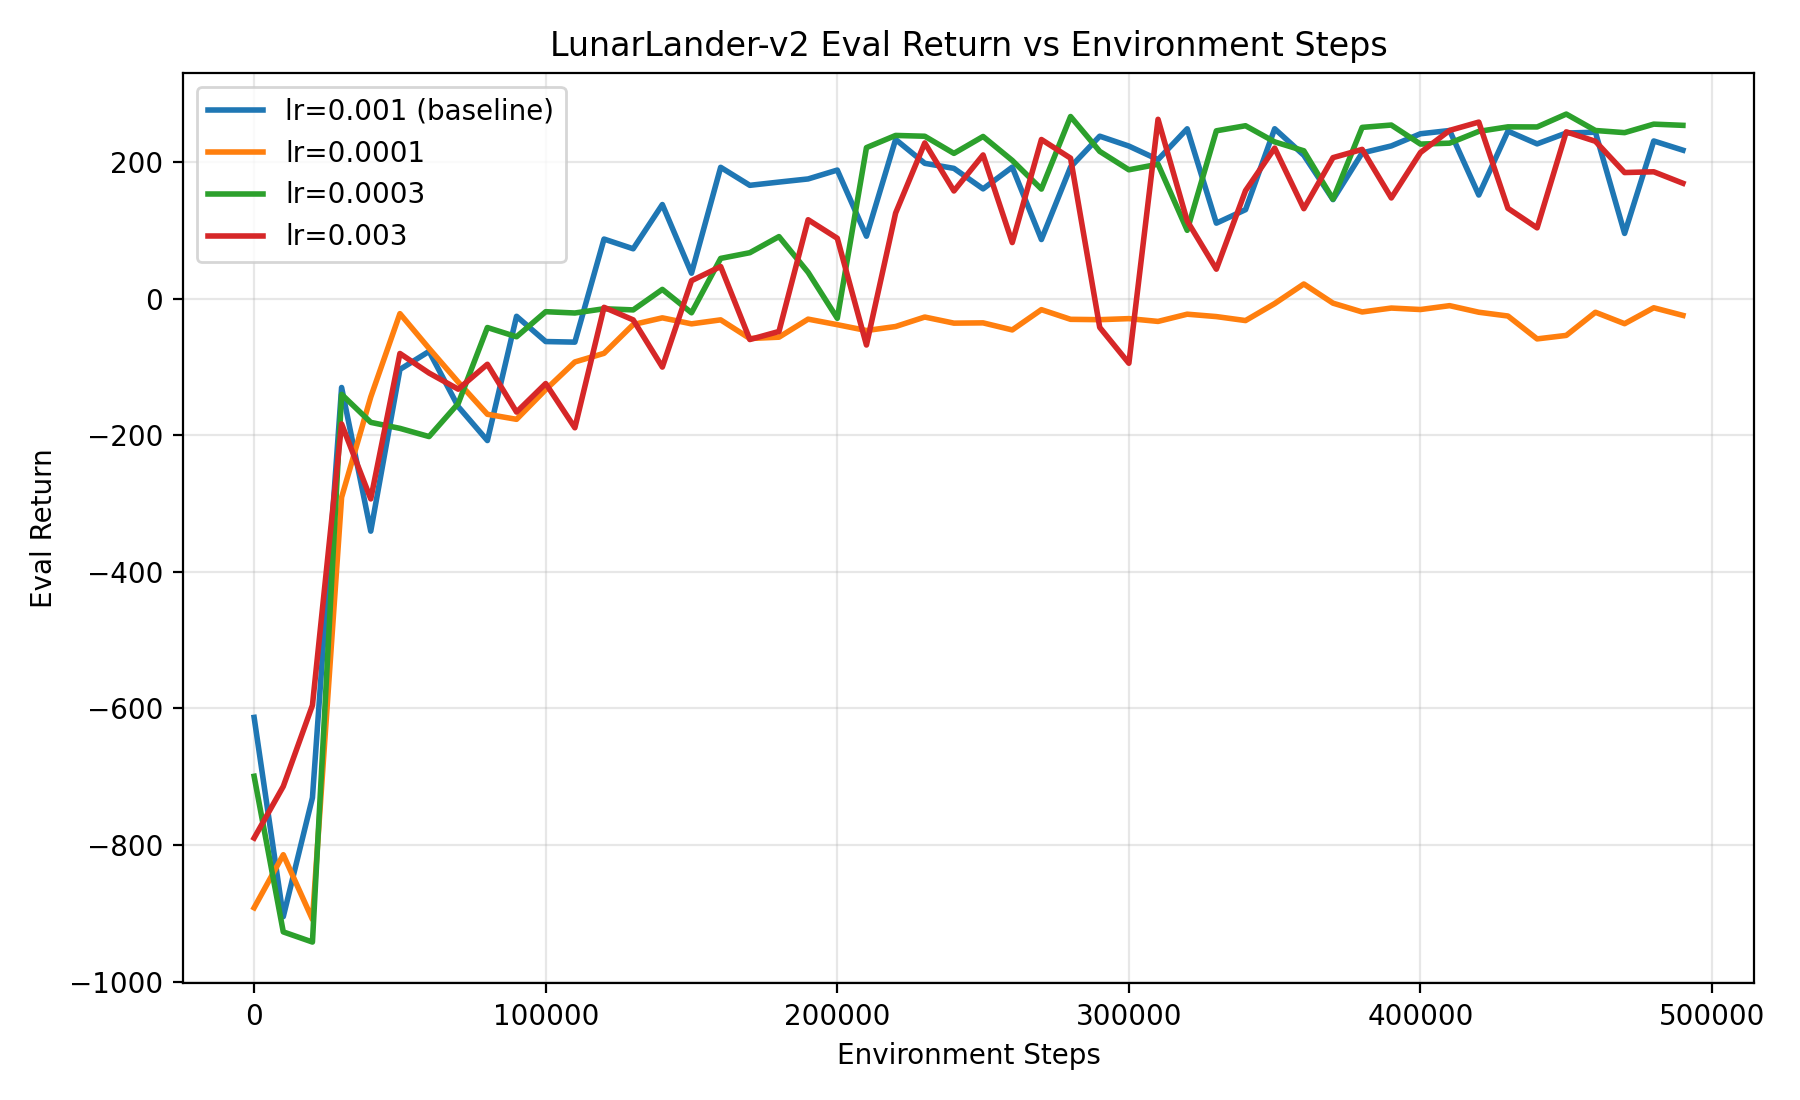
\includegraphics[width=0.9\linewidth]{lunarlander_hyperparameter_eval_return.png}
    \caption{LunarLander-v2 evaluation return for four learning rates: 0.001 (baseline), 0.0001, 0.0003, and 0.003. Smaller learning rates were generally more stable but slower, while larger learning rates improved faster initially but were less stable.}
\end{figure}

\section{Soft Actor-Critic}

\subsection{Sanity Check on InvertedPendulum-v4}
I implemented the SAC training loop, including critic updates, entropy-regularized actor updates, soft target-network updates, and replay-based off-policy learning. On InvertedPendulum-v4 with fixed temperature, the agent reached an evaluation return of 1000, indicating that it learned to balance the pendulum for the full episode.

\begin{figure}[H]
    \centering
    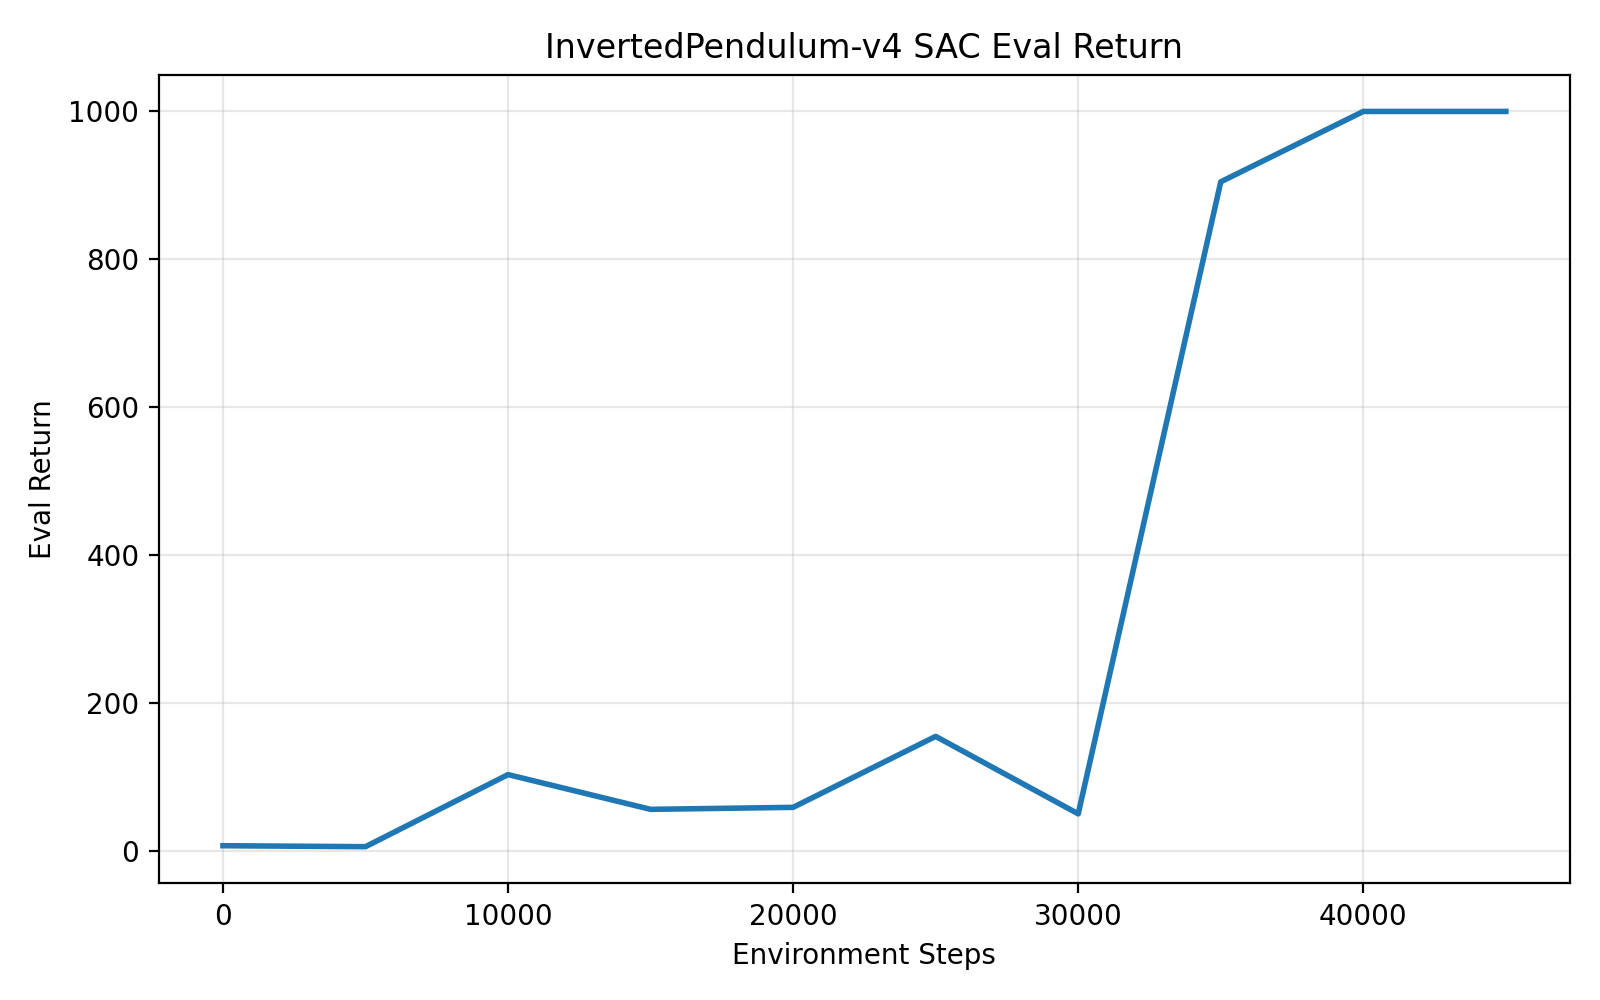
\includegraphics[width=0.8\linewidth]{invertedpendulum_sac_eval_return.png}
    \caption{InvertedPendulum-v4 SAC evaluation return versus environment steps.}
\end{figure}

\subsection{Automatic Temperature Tuning}
I also implemented automatic temperature tuning by optimizing the log-temperature parameter against a target entropy objective. In this run, the auto-tuned variant was less stable than the fixed-temperature baseline: it briefly improved but did not consistently reach the near-1000 return achieved by the fixed-temperature run.

\begin{figure}[H]
    \centering
    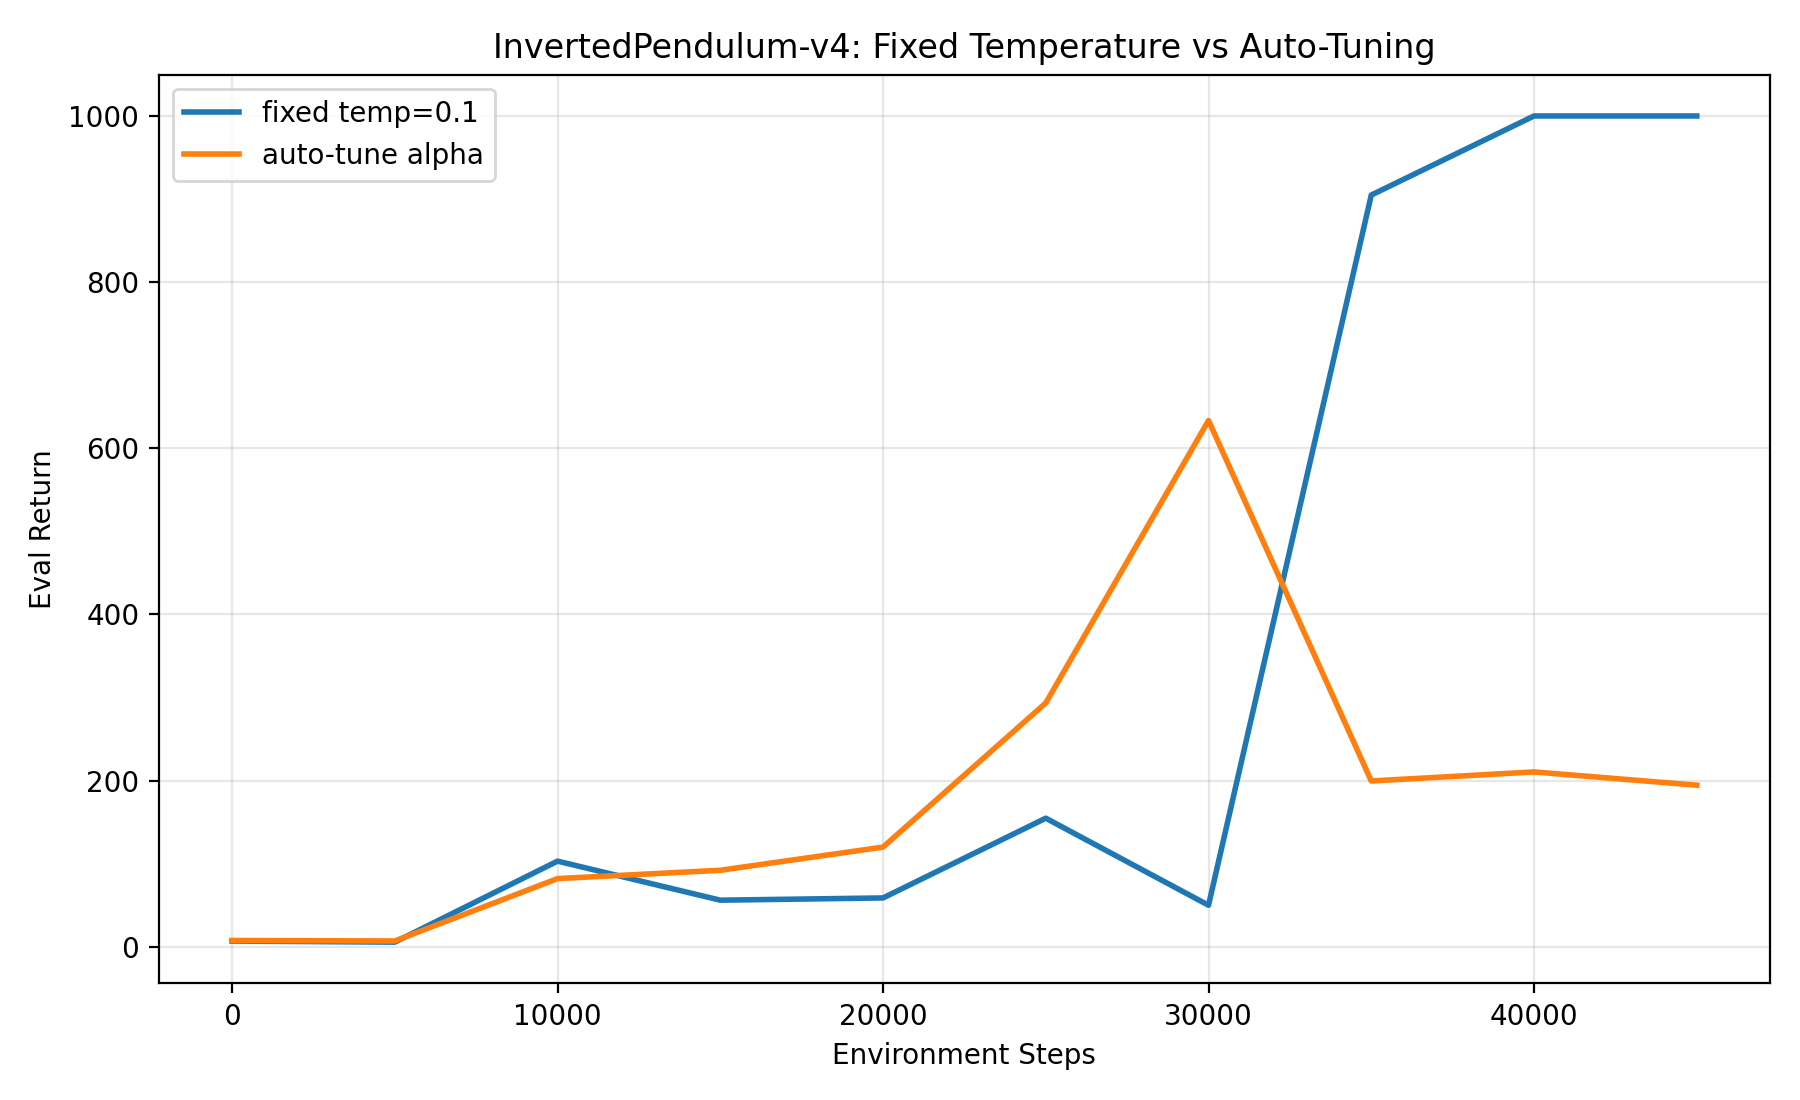
\includegraphics[width=0.8\linewidth]{invertedpendulum_sac_vs_autotune_eval_return.png}
    \caption{InvertedPendulum-v4 comparison between fixed temperature and automatic temperature tuning.}
\end{figure}

\begin{figure}[H]
    \centering
    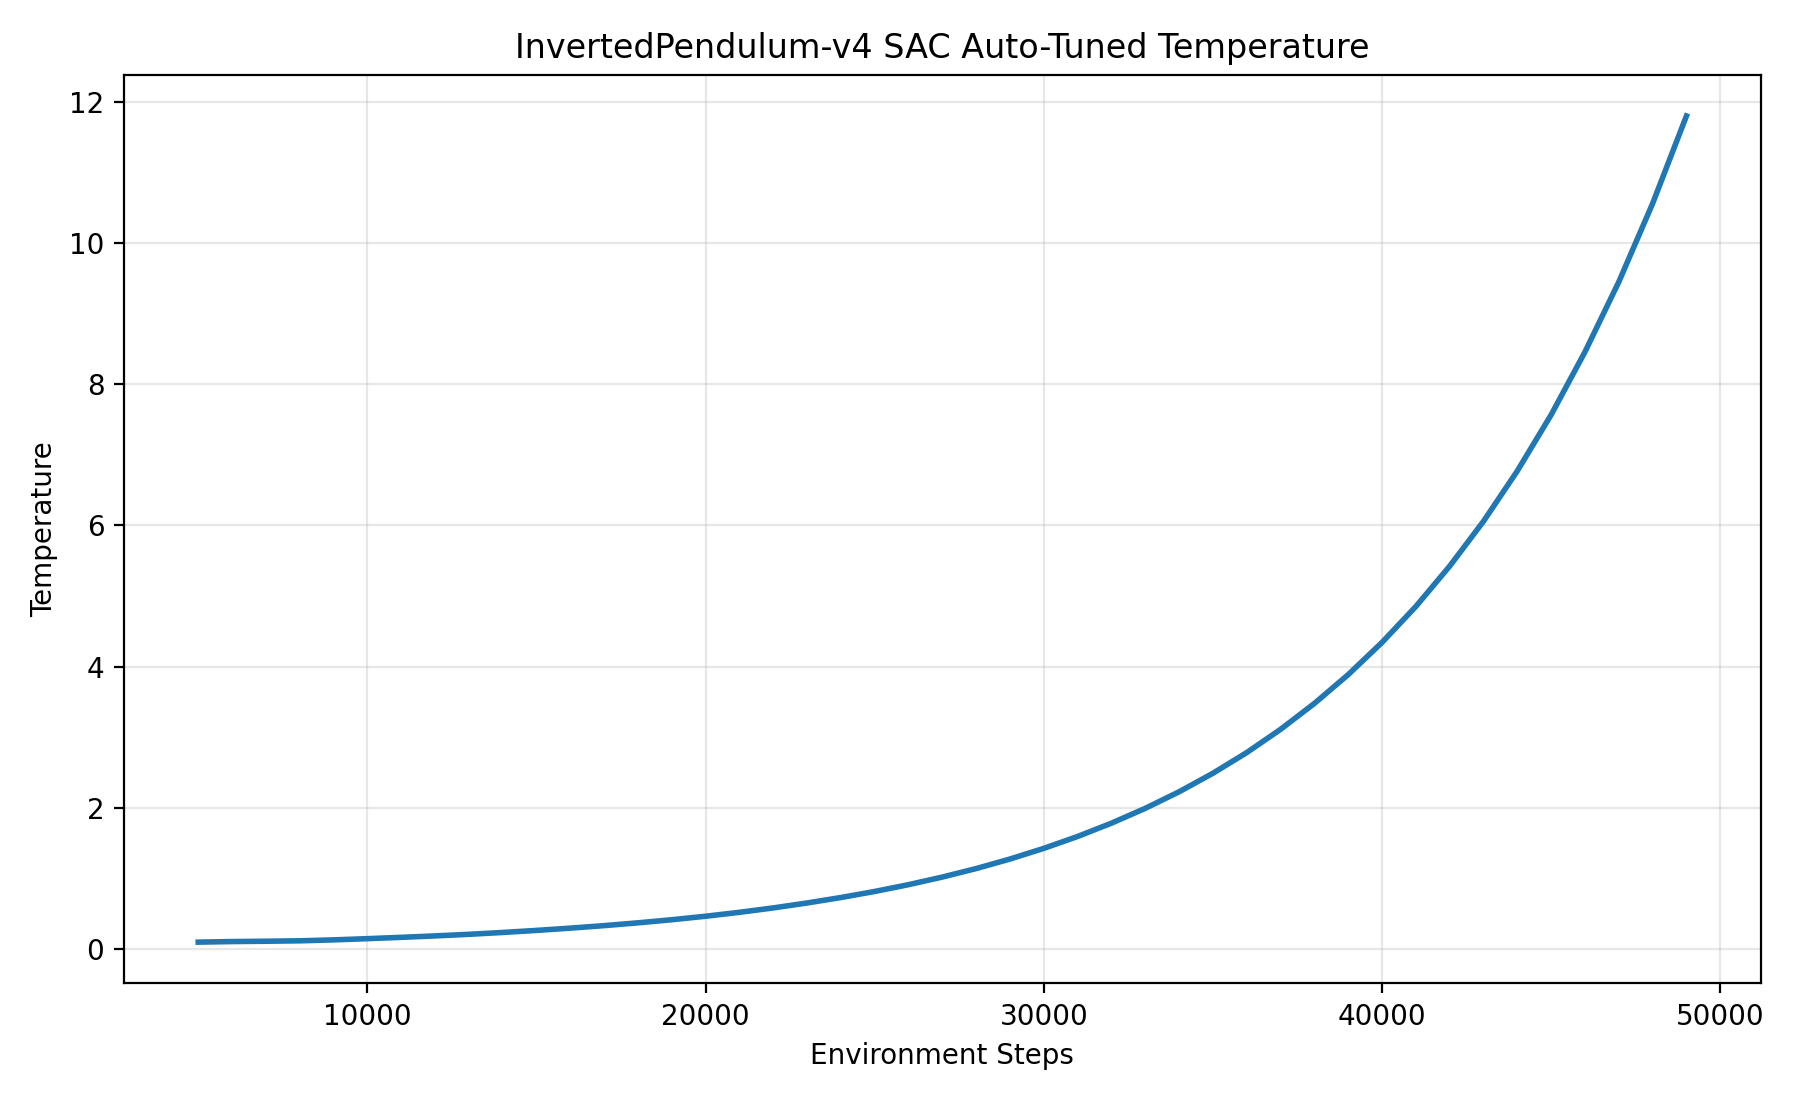
\includegraphics[width=0.8\linewidth]{invertedpendulum_sac_autotune_temperature.png}
    \caption{Automatically tuned temperature during InvertedPendulum-v4 training.}
\end{figure}

\subsection{Single-Q versus Clipped Double-Q on Hopper-v4}
To study the effect of multiple critics, I compared a single-Q SAC agent against clipped double-Q SAC on Hopper-v4. The clipped double-Q variant substantially outperformed the single-Q baseline. In my runs, clipped double-Q reached a best evaluation return of approximately 3237.5, while the single-Q version peaked near 1001.9. This is consistent with the motivation for clipped double-Q: taking the minimum over two target critics reduces overestimation bias and generally improves stability.

\begin{figure}[H]
    \centering
    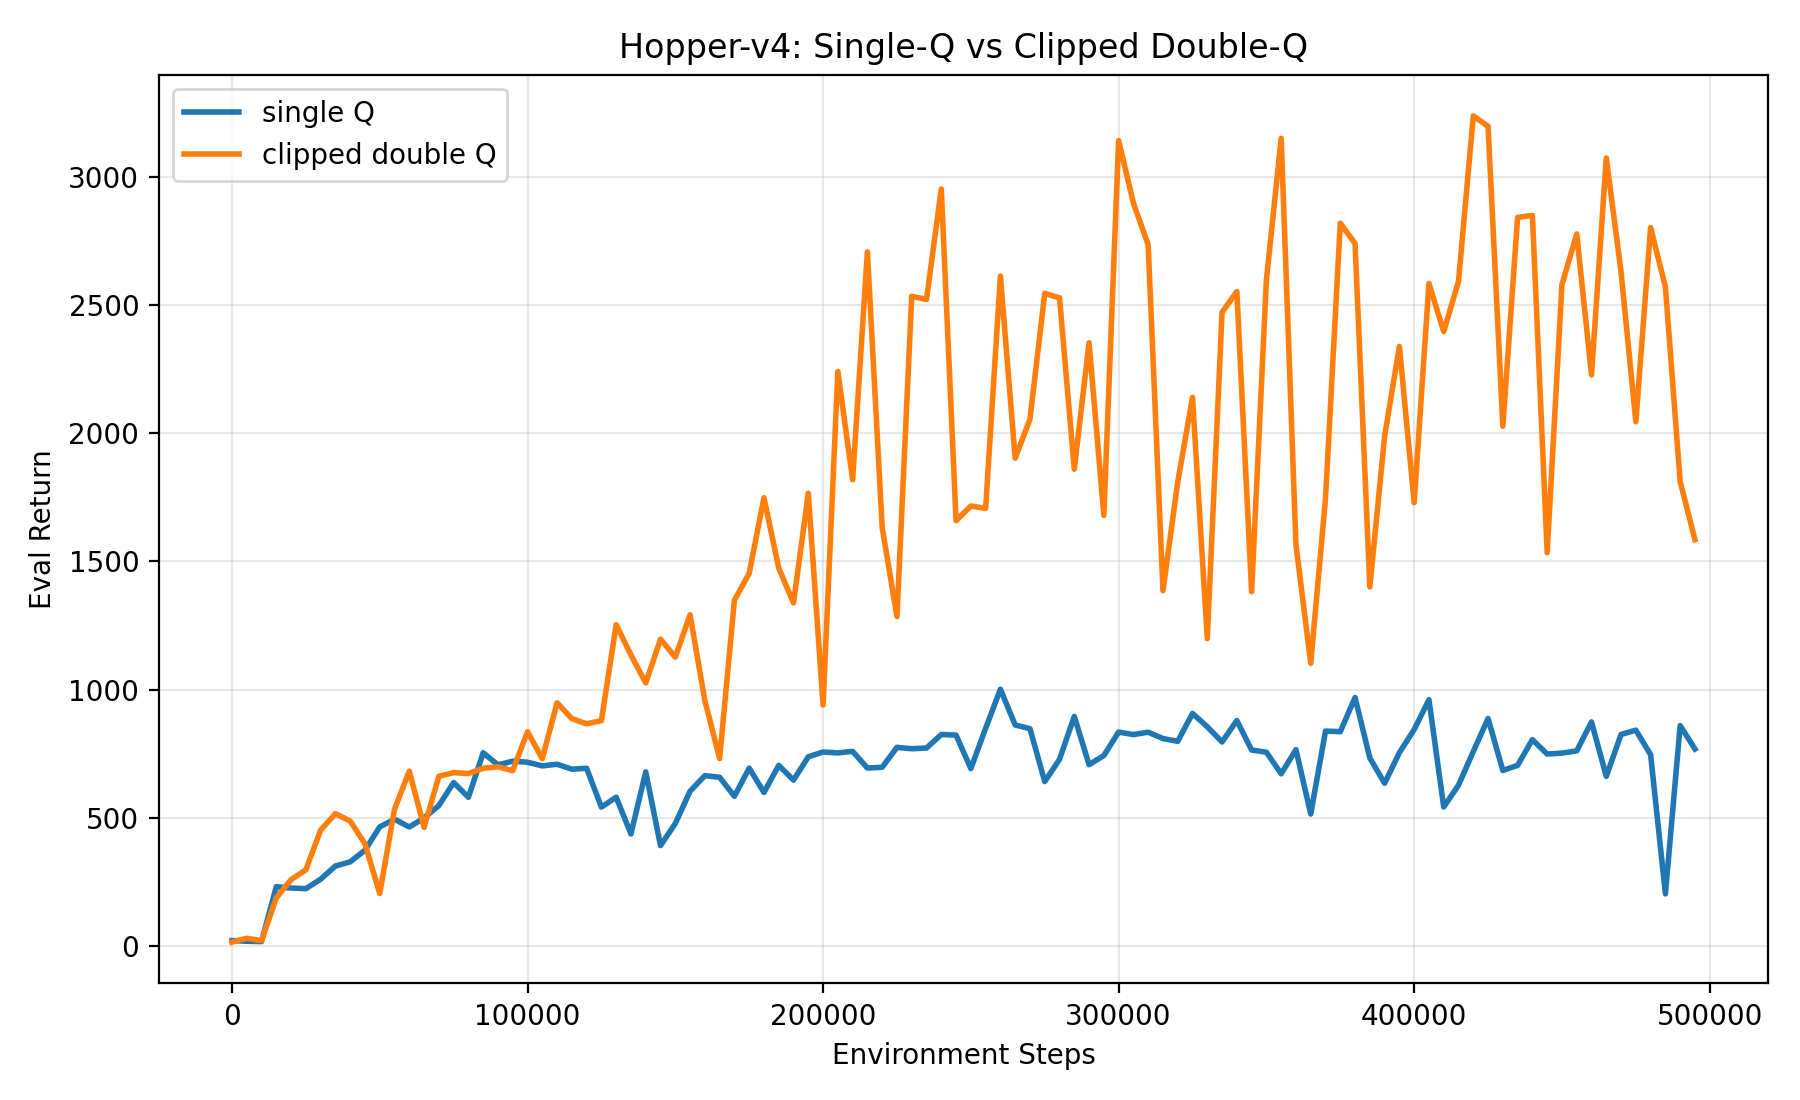
\includegraphics[width=0.9\linewidth]{hopper_singleq_vs_clipq_eval_return.png}
    \caption{Hopper-v4 comparison of single-Q SAC and clipped double-Q SAC.}
\end{figure}

\subsection{HalfCheetah-v4}
For HalfCheetah-v4, I compared the fixed-temperature SAC agent against the auto-tuned-temperature SAC agent on the same environment and training budget. In the final successful runs, both methods learned strong policies, but the auto-tuned variant performed slightly better. The fixed-temperature agent reached a best and final evaluation return of approximately 9182.4, while the auto-tuned run reached approximately 9791.6 by the end of training.

\begin{figure}[H]
    \centering
    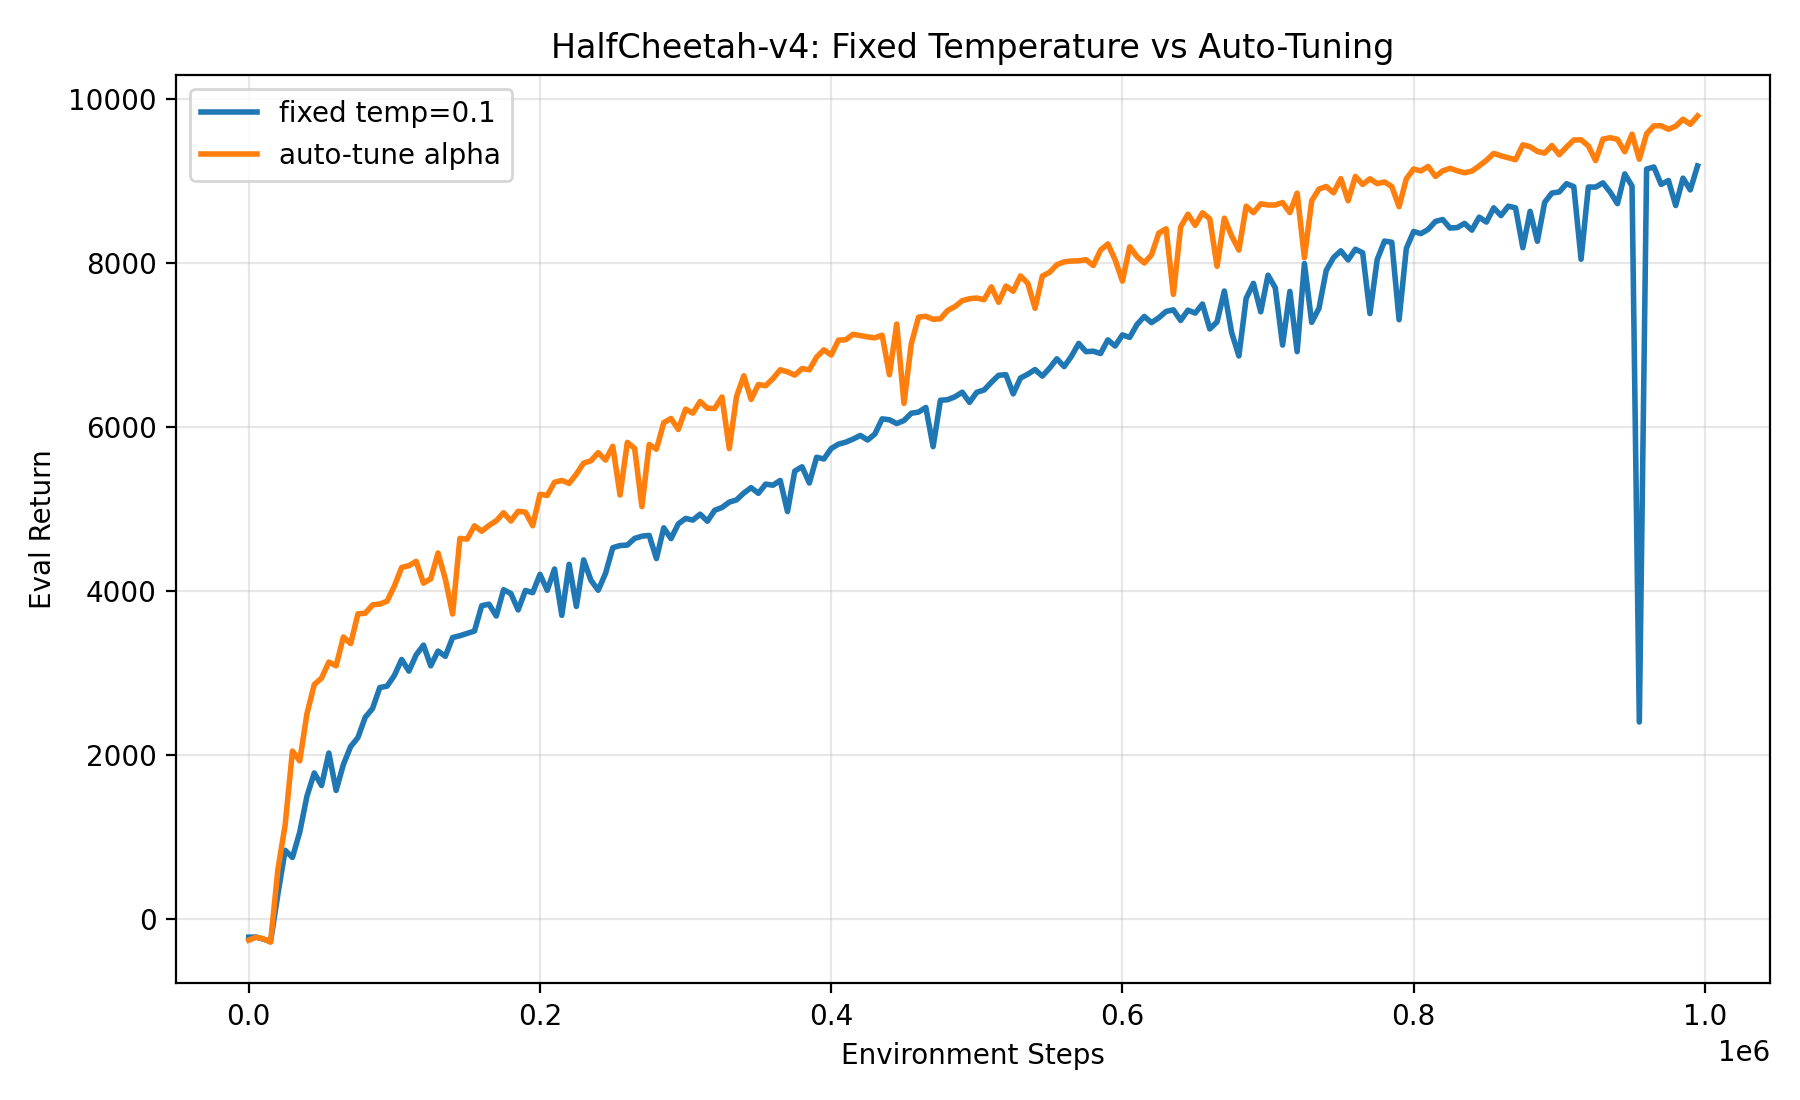
\includegraphics[width=0.9\linewidth]{halfcheetah_sac_vs_autotune_eval_return.png}
    \caption{HalfCheetah-v4 evaluation return for fixed-temperature SAC and auto-tuned SAC.}
\end{figure}

\begin{figure}[H]
    \centering
    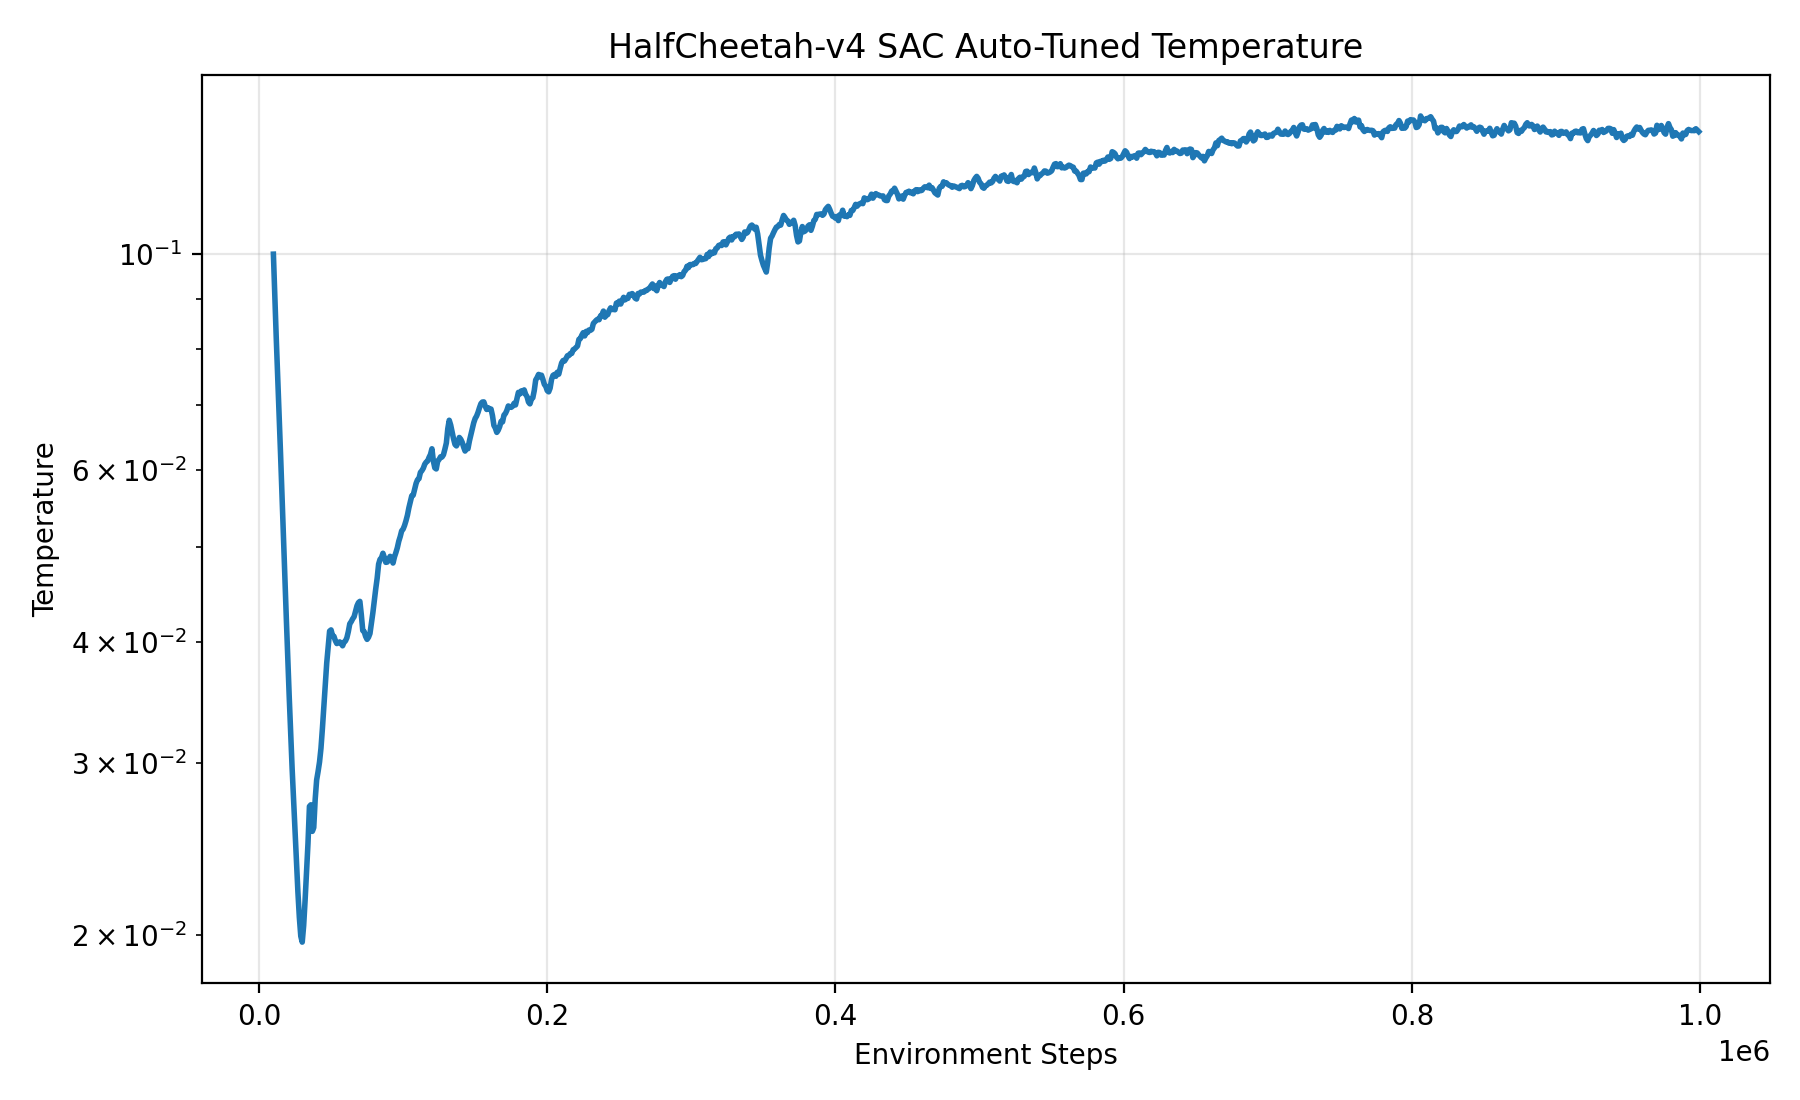
\includegraphics[width=0.8\linewidth]{halfcheetah_sac_autotune_temperature.png}
    \caption{Temperature during HalfCheetah-v4 auto-tuned SAC training (log scale).}
\end{figure}

In this experiment, automatic temperature tuning improved slightly over the fixed-temperature baseline. The learned temperature stayed well-behaved throughout training and converged to a small value near 0.13 rather than exploding. This suggests that the temperature objective adapted the entropy bonus to a reasonable scale for HalfCheetah-v4, allowing the policy to maintain useful exploration early in training while still focusing on reward maximization later. Empirically, both runs were strong, but the auto-tuned version achieved the higher final return in this run.

\section{Summary}
Across the DQN experiments, the implementation passed the CartPole-v1 sanity check, achieved solid LunarLander-v2 performance with double DQN, and produced strong Atari performance on MsPacman-v0. Across the SAC experiments, the fixed-temperature implementation solved InvertedPendulum-v4, clipped double-Q clearly improved Hopper-v4 performance relative to a single-Q baseline, and on HalfCheetah-v4 the auto-tuned SAC agent slightly outperformed the fixed-temperature baseline in the final successful run.

\end{document}
